\section{Organizational Structure}

\subsection{General Structure}

The organizational structure of NIST includes six laboratories and several extramural programs (Figure \ref{fig:nist-organization-chart}) \cite{nist2016organization}.

NIST facilities include:

\begin{itemize}
    \item Center for Nanoscale Science and Technology (CNST)
    \item Communications Technology Laboratory (CTL)
    \item Engineering Laboratory (EL)
    \item Information Technology Laboratory (ITL)
    \item Material Measurement Laboratory (MML)
    \item NIST Center for Neutron Research (NCNR)
    \item Physical Measurement Laboratory (PML)
\end{itemize}

The external programs include:

\begin{itemize}
    \item Baldrige Performance Excellence Program
    \item Hollings Manufacturing Extension Partnership (MEP)
    \item Technology Innovation Program (TIP)
\end{itemize}

\begin{figure}[ht]
  \centering
  \includegraphics[scale=0.50]{figures/nist-organization-chart}
  \caption{NIST Organization Chart \cite{nist2016orgchart}}
  \label{fig:nist-organization-chart}
\end{figure}

During this internship, I had the opportunity to work within the Information Technology Laboratory (ITL), more precisely in its Software and Systems Division (SSD). More details are given on the ITL and the SSD in the following sections.

\clearpage

\subsection{Information Technology Laboratory}

``The Information Technology Laboratory (ITL), one of seven research laboratories within the National Institute of Standards and Technology (NIST), develops and deploys standards, tests, and metrics to make our information systems more secure, usable, interoperable, and reliable. As a world-class measurement and testing laboratory encompassing a wide range of areas of computer science, mathematics, statistics, and systems engineering, its research program supports NIST’s mission to promote U.S. innovation and industrial competitiveness by advancing measurement science, standards, and related technology through research and development in ways that enhance economic security and improve our quality of life.

ITL collaborates with other NIST laboratories, the Department of Commerce, other government agencies, the U.S. private sector, standards development organizations, and other national and international stakeholders in both the development and application of new information technologies to help meet national priorities. ITL is called upon to address national priorities due to its reputation as a globally recognized and trusted source of high-quality, independent, and unbiased research and data, and as a trusted third-party convener. The resulting measurement and standards infrastructure catalyzes innovation in IT and IT-related measurement science which drive progress across scientific, technology, and commercial applications.

ITL’s strategy is to maximize the benefits of IT to society through a balanced IT measurement science and standards portfolio of three major activities: fundamental research in mathematics, statistics, and IT; applied IT research and development; and standards development and technology transfer'' \cite{nist2016itlpresentation}.

ITL's organizational structure is presented in Figure \ref{fig:nist-itl-organization-chart}. 

\begin{figure}[ht]
  \centering
  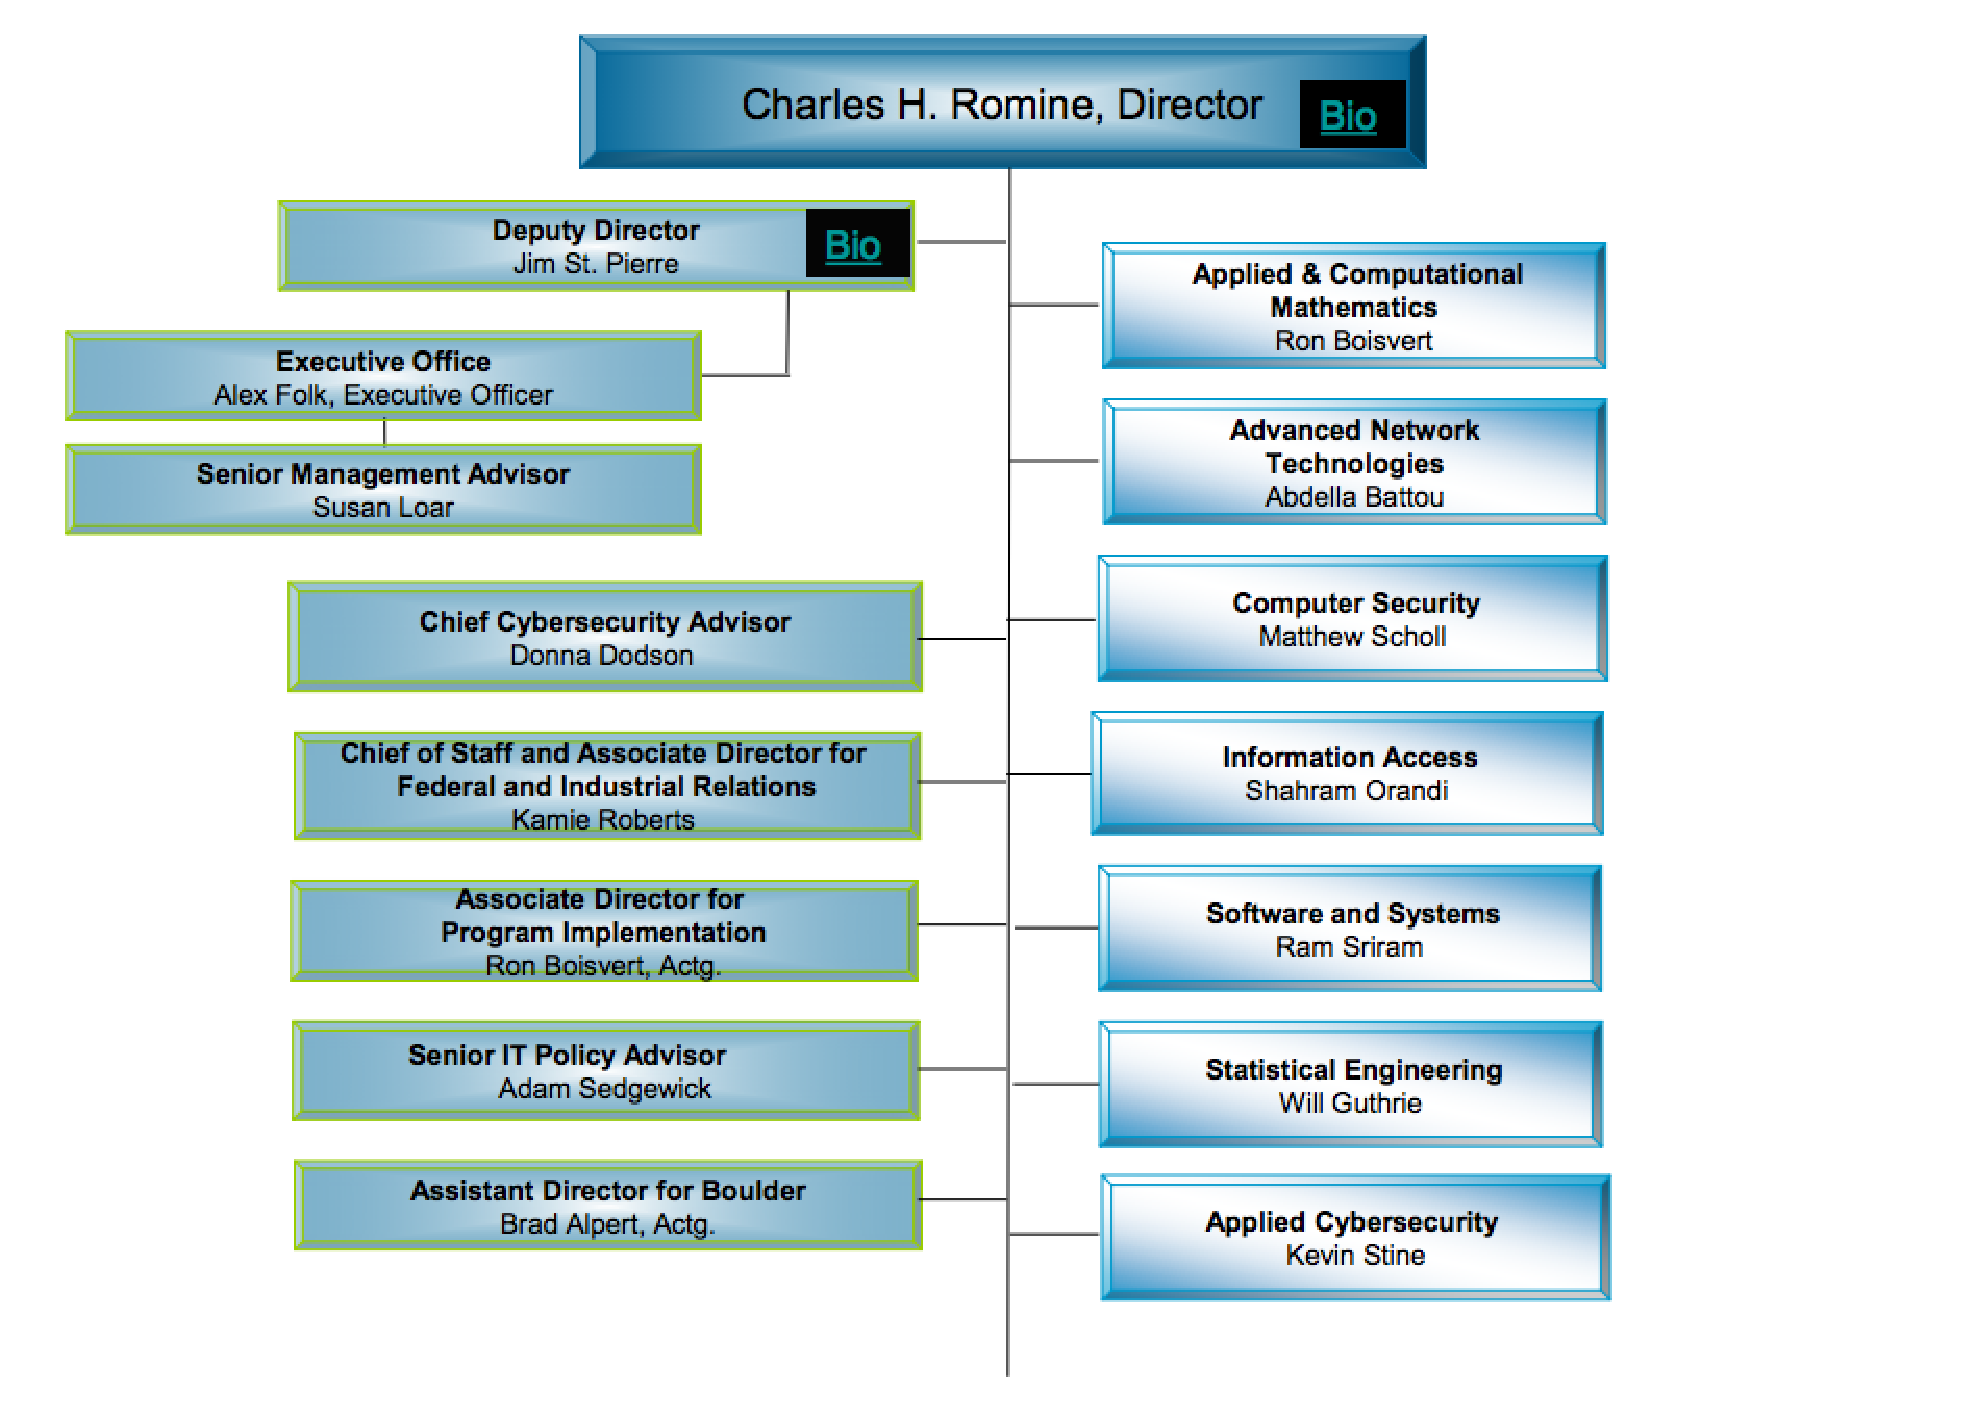
\includegraphics[scale=0.50]{figures/nist-itl-organization-chart}
  \caption{Information Technology Laboratory (ITL) Organization Chart \cite{nist2016itlorgchart}}
  \label{fig:nist-itl-organization-chart}
\end{figure}

\clearpage

\subsection{Software and Systems Division}

``The mission of the Software and Systems Division (SSD) is to work with industry, academia and other government agencies to accelerate the development and adoption of correct, reliable, testable software, leading to increased trust and confidence in deployed software; promulgate methods to develop better standards and testing tools for today's software infrastructures and tomorrow's next-generation software systems; advance the state of the art of software testing by developing scientifically rigorous, breakthrough techniques to automatically generate tests that are cheaper to develop and more comprehensive; lead efforts for conformance testing, especially at the early stage of standards development; develop integrated test environments to coalesce systems; facilitates the transfer of these activities and technologies into national infrastructures and commercial sectors'' \cite{nist2016ssdpresentation}.

The Software and Systems Division comprises the four following groups (see fig. \ref{fig:nist-division-organization-chart}):

\begin{itemize}
    \item Software Quality Group
    \item Information Systems Group
    \item Systems Interoperability Group
    \item Cyber Infrastructure Group
\end{itemize}

I was assigned to the Software Quality Group, which develops tools, methods, and related models for improving the process of ensuring that software behaves correctly and for identifying software defects, thus helping industry improve the quality of software development and maintenance \cite{nist2016ssdprojects}. Each group is managing multiple programs and projects. I joined the Software Assurance Metrics And Tool Evaluation (\gls{samate}) team.

\begin{figure}[ht]
  \centering
  \includegraphics[scale=0.48]{figures/nist-division-organization-chart}
  \caption{Software and Systems Division (SSD) Organization Chart}
  \label{fig:nist-division-organization-chart}
\end{figure}

\subsection{SAMATE Project}

The NIST \gls{samate} project began in Fall 2004. It is dedicated to improving software assurance by developing methods to enable software tool evaluations, measuring the effectiveness of tools and techniques, and identifying gaps in tools and methods. The scope of the \gls{samate} project is broad: ranging from operating systems to firewalls, SCADA to web applications, source code security analyzers to correct-by-construction methods \cite{nist2016samatepresentation}.

The \gls{samate} project consists of two parts:

\begin{itemize}
    \item the development of metrics for the effectiveness of software security assessment (SSA) tools, and
    \item assess current SSA methods and tools in order to identify deficiencies which can lead to software product failures and \glspl{vulnerability}. 
\end{itemize}

\clearpage

\subsubsection{Support Tool Evaluation}

One of \gls{samate}'s goals is to establish a methodology for evaluating software assurance tools by developing tool specifications, test plans, and test sets. The results provide information for tool developers to improve tools, for users to make informed choices about acquiring and using software tools, and for interested parties to understand tool capabilities. \gls{samate}'s efforts include:

\begin{itemize}
    \item Source Code Security Analyzers - This class of software examines source code files for security \glspl{weakness} and potential \glspl{vulnerability}. \gls{samate} published a specification as NIST Special Publication 500-268 v1.1 \cite{black2007source}.
    \item Web \Gls{vulnerability} Scanners - These tools crawl a web application's pages and search for \glspl{vulnerability} by simulating attacks on it. A specification is published as NIST Special Publication 500-269. A test framework for web application scanners appeared in a paper entitled "Building a Test Suite for Web Application Scanners" and published in 41st Hawaii Internation Conference on System Sciences (HICSS), January 2008.
    \item Binary Code Scanners - Similar to source code security analyzers, this class of tool analyzes a compiled binary application, including libraries, and provides a report of code \gls{weakness} over the entire application.
    \item The \gls{sard} \cite{nist2016sard} - A community repository of example code and other artifacts to help end users evaluate tools and developers test their methods.
    \item Static Analysis Tools Exposition (\gls{sate}) - The goals of these expositions are to enable empirical research based on large test sets, encourage improvement of tools, and speed tool adoption by objectively demonstrating their use on real software.
\end{itemize}

\subsubsection{Workshops}

In order to bring a community together, help learn and share results, \gls{samate} hosts or co-hosts workshops, conferences sessions, and other meetings. Among the latest:

\begin{itemize}
    \item Software Measures and Metrics to Reduce Security \Glspl{vulnerability} (SwMM-RSV) Workshop, NIST, Gaithersburg, Maryland, July 2016.
    \item Static Analysis Tool Exposition (\gls{sate}) V Workshop, NIST, Gaithersburg, Maryland, March 2014.
    \item Metrics and Standards for Software Testing (MaSST) Workshop, NIST, Gaithersburg, Maryland, June 2012. 
    \item Static Analysis Tool Exposition (\gls{sate}) IV Workshop, co-located with the Spring 2012 Software Assurance Forum, MITRE, McLean, Virginia, March 2012.
    \item Static Analysis Tool Exposition (\gls{sate}) 2010 Workshop, co-located with the 13\textsuperscript{th} semi-annual Software Assurance Forum, NIST, Gaithersburg, Maryland, October 2010.
    \item Static Analysis Tool Exposition (\gls{sate}) 2009 Workshop, co-located with the 11\textsuperscript{th} semi-annual Software Assurance Forum, Arlington, Virginia, November 2009.
    \item Static Analysis Workshop (SAW), including Static Analysis Tool Exposition (\gls{sate}) 2008 reports, co-located with PLDI, Tucson, Arizona, June 2008.
    \item Static Analysis Summit II (SASII) in conjunction with SIGAda, Fairfax, Virginia, November 2007.
    \item Static Analysis Summit I (SAS), Gaithersburg, Maryland, June 2006.
    \item Workshop on Software Security Assurance Tools, Techniques, and Metrics (SSATTM), Long Beach, California, November 2005.
    \item Workshop on Defining the State of the Art in Software Security Tools, Gaithersburg, Maryland, Aug 2005.
\end{itemize}

\clearpage